
\section{Annexe : Code réalisé pour le tutoriel sur les tests d'hypothèse}

\begin{lstlisting}[language=R]
#######################
# Cas ou H0 est vraie 
####################### 

# On va considerer deux populations qui ont exactement
# les memes parametres : les deux sont uniformement 
# distribuees entre 0 et 1. Les deux populations ont
# donc la meme moyenne, en l'occurrence 0.5. 
# Puis nous allons faire une experience : 
# - tirer un petit echantillon dans chaque population
# - calculer la moyenne observee dans l'echantillon 1,
#   puis celle observee dans l'echantillon 2. On 
#   n'obtiendra pas exactement 0.5 ni pour l'une ni pour 
#   l'autre.
# - calculer la difference entre les deux moyennes 
#   d'echantillons. Appelons d cette difference.

tirerEchantillonPop1H0 <- function(n) {
	vraieMoyenne <- 0.5
	plageDeDispersion <- 1.0
	min <- vraieMoyenne - plageDeDispersion/2.0
	max <- vraieMoyenne + plageDeDispersion/2.0
	ech <- runif(n, min, max)
	return(ech)
}

tirerEchantillonPop2H0 <- function(n) {
	vraieMoyenne <- 0.5
	plageDeDispersion <- 1.0
	min <- vraieMoyenne - plageDeDispersion/2.0
	max <- vraieMoyenne + plageDeDispersion/2.0
	ech <- runif(n, min, max)
	return(ech)
}

# Ecrire ici le code permettant de faire une "experience"
# c'est a dire tirer un echantillon de taille 20 dans 
# chaque population et mesurer la difference d observee
# entre les 2 moyennes d'echantillon.
pop1 <- tirerEchantillonPop1H0(20)
pop2 <- tirerEchantillonPop2H0(20)

mean(pop1)
mean(pop2)
abs(mean(pop1) - mean(pop2))
abs(mean(tirerEchantillonPop1H0(20)) - mean(tirerEchantillonPop2H0(20)))

# Si 1000 etudiants font independamment cette experience,
# chaque etudiant aura des echantillons differents et donc
# chacun aura une valeur differente pour d. Si nous 
# mettons toutes ces 1000 valeurs ensemble dans un vecteur
# (appele diffMoyH0), quelle sera la moyenne de ce vecteur ?

diffMoyH0 = c()

for(i in  1:1000)
{
	diffMoyH0 = c(diffMoyH0, abs(mean(tirerEchantillonPop1H0(20)) - mean(tirerEchantillonPop2H0(20))))
}

# On affiche la moyenne totale.
mean(diffMoyH0)

# On affiche les 1000 valeurs sur un histogramme.
plot(diffMoyH0)
abline(h=mean(diffMoyH0), col="red")

\end{lstlisting}

On obtient une moyenne de 0,07.

\begin{lstlisting}[language=R]

#######################
# Cas ou H1 est vraie 
####################### 

# On va voir comment se comporte notre indicateur quand 
# les deux populations n'ont pas la meme moyenne
# (mais ont tout de meme la meme dispersion)
# eg . pop1 comprise entre 0.0 et 1.0
#   et pop2 comprise entre 0.2 et 1.2 

tirerEchantillonPop1H1 <- function(n) {
vraieMoyenne <- 0.5
plageDeDispersion <- 1.0
min <- vraieMoyenne - plageDeDispersion/2.0
max <- vraieMoyenne + plageDeDispersion/2.0
ech <- runif(n, min, max)
return(ech)
}

tirerEchantillonPop2H1 <- function(n) {
vraieMoyenne <- 0.7
plageDeDispersion <- 1.0
min <- vraieMoyenne - plageDeDispersion/2.0
max <- vraieMoyenne + plageDeDispersion/2.0
ech <- runif(n, min, max)
return(ech)
}


# Ecrire ici le code pour faire les 1000 experiences 
# comme precedemment, en nommant cette fois le vecteur
# diffMoyH1. Calculez sa moyenne et tracez son histogramme.

diffMoyH1 = c()

for(i in  1:1000)
{
	diffMoyH1 = c(diffMoyH1, abs(mean(tirerEchantillonPop1H1(20)) - mean(tirerEchantillonPop2H1(20))))
}

# On affiche la moyenne totale.
mean(diffMoyH1)

# On affiche les 1000 valeurs sur un histogramme.
plot(diffMoyH1)
abline(h=mean(diffMoyH1), col="red")

\end{lstlisting}

On obtient une moyenne de 0,2.

\begin{figure}[htbp]
	\begin{center}
		% remplacez par votre figure 
		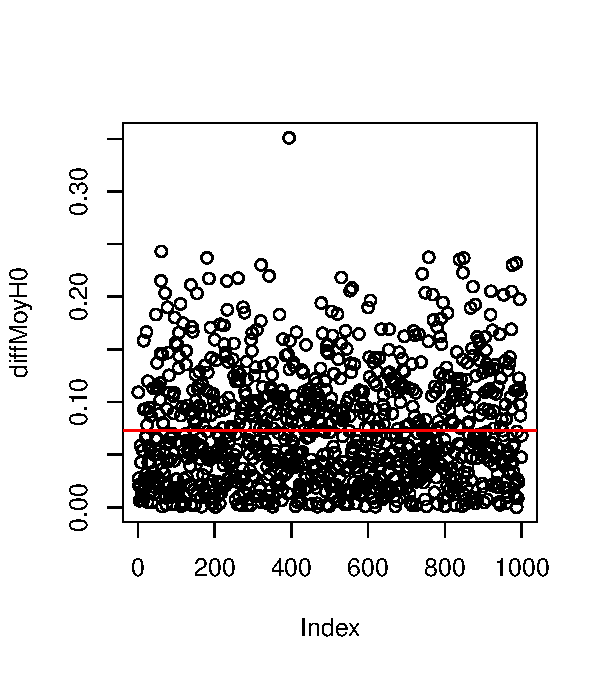
\includegraphics[width=12cm]{diffMoy.pdf}
		\caption{Graphique représentant diffMoyH0 et diffMoyH1 ainsi que leur moyenne.}
		\label{fig:diffMoy}
	\end{center}
\end{figure}


Placons nous maintenant dans le cas ou l'on ait fait
une seule experience.

Ecrire le code pour evaluer la plausibilite de H0: "les deux 
echantillons proviennent de deux populations qui ont la meme moyenne".

\begin{lstlisting}[language=R]
cMean <- function(v1, v2)
{
	return(abs(mean(v1) - mean(v2)))
}
sameMean <- function(v1, v2)
{
	return(cMean(v1, v2) < 0.1)
}

sameMean(tirerEchantillonPop1H0(20), tirerEchantillonPop2H0(20))
sameMean(tirerEchantillonPop1H1(20), tirerEchantillonPop2H1(20))

x1 <- c(0.97050525, 0.13734516, 0.80793033, 0.05207726, 0.62629180, 0.93485856,
0.58220744, 0.65935145, 0.76467195, 0.73512414, 0.45139560, 0.93225380,
0.53790595, 0.99845675, 0.31035081, 0.43082815, 0.15475353, 0.42647652,
0.65676067, 0.74186048)
x2 <- c(0.33565036, 0.28830545, 0.51556544, 0.93223089, 0.29192576, 0.43505823,
0.63127002, 0.86082799, 0.56533392, 0.19083212, 0.13087779, 0.09849703,
0.98921291, 0.91480756, 0.78556552, 0.33859160, 0.88482223, 0.76701274,
0.24190609, 0.46251866)

cMean(x1, x2)
sameMean(x1, x2)
\end{lstlisting}

Ici, sameMean(x1, x2) retourne "TRUE", ce qui signifie que les deux échantillons ont une moyenne proche l'une de l'autre.

\begin{figure}[htbp]
	\begin{center}
		% remplacez par votre figure 
		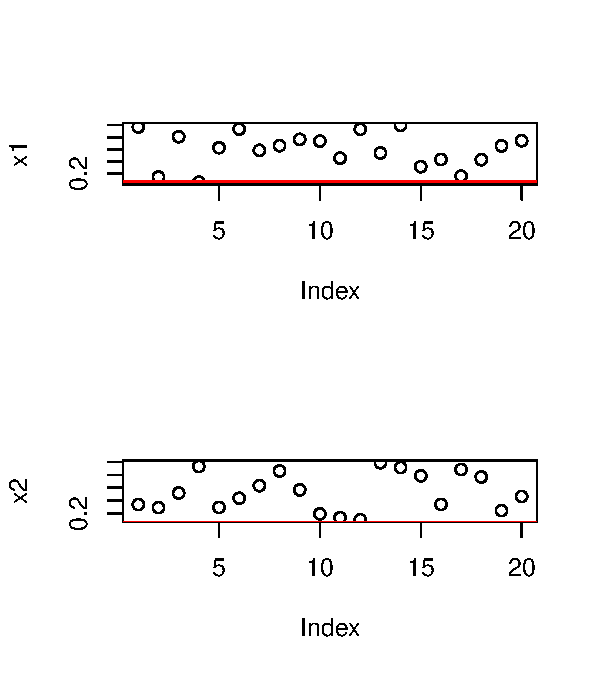
\includegraphics[width=12cm]{x1-x2-1.pdf}
		\caption{Graphique représentant x1 and x2 ainsi que leur moyenne.}
		\label{fig:x1-x2-1}
	\end{center}
\end{figure}

\begin{lstlisting}[language=R]
x1 <- c(0.41236444, 0.28422821, 0.15093798, 0.05885328, 0.25514435, 0.63026931,
0.56325462, 0.76304859, 0.56523993, 0.92535660, 0.10898729, 0.51579642,
0.07223967, 0.53483839, 0.52516575, 0.20250815, 0.89634680, 0.53879059,
0.58736912, 0.53945749)
x2 <- c(1.0809923, 0.5772333, 0.7252340, 1.1529082, 1.0924642, 0.6046166, 0.9495800,
0.3019857, 0.7701195, 1.0746508, 0.3928894, 1.0885017, 0.5101510, 1.1871599,
0.7953318, 0.5711237, 0.5505642, 0.9854085, 0.5105643, 0.9601635)

cMean(x1, x2)
sameMean(x1, x2)
\end{lstlisting}

Ici, sameMean(x1, x2) retourne "FALSE", ce qui signifie que les deux échantillons ont une moyenne bien différente l'une de l'autre.

\begin{figure}[htbp]
	\begin{center}
		% remplacez par votre figure 
		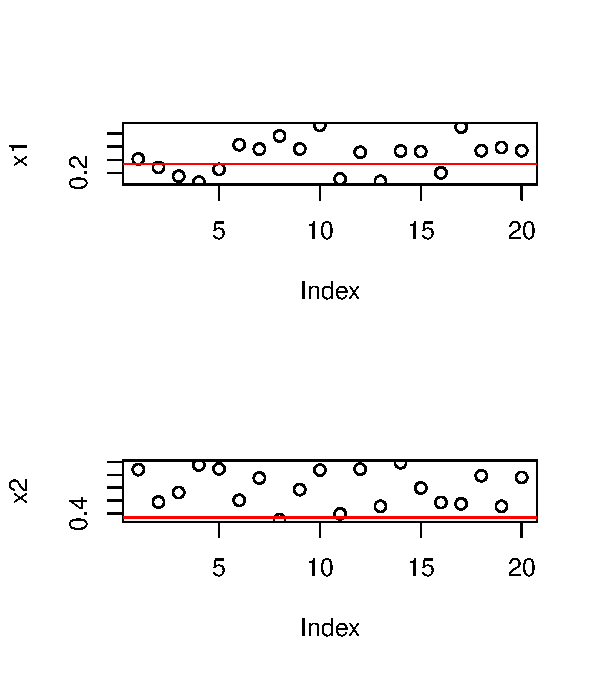
\includegraphics[width=12cm]{x1-x2-2.pdf}
		\caption{Graphique représentant x1 and x2 ainsi que leur moyenne.}
		\label{fig:x1-x2-2}
	\end{center}
\end{figure}


Incorporez également les histogrammes obtenus sous forme de figures. Indiquez vos conclusions sur les deux paires d'échantillons. 
